\documentclass{article}
%----------------------------------------------------------------------------------------
%	PACKAGES AND OTHER DOCUMENT CONFIGURATIONS
\usepackage[utf8]{inputenc}
\usepackage{graphicx}
\usepackage{tabularx}
\usepackage[export]{adjustbox}
\usepackage{paralist}
\usepackage{wrapfig}
\usepackage{geometry}
 \geometry{
 a4paper,
 total={170mm,257mm},
 left=20mm,
 top=20mm,
 }
%----------------------------------------------------------------------------------------

\newcommand*{\plogo}{\fbox{$\mathcal{PL}$}} % Generic publisher logo

%----------------------------------------------------------------------------------------
%	TITLE PAGE
%----------------------------------------------------------------------------------------

\newcommand*{\titleGP}{\begingroup % Create the command for including the title page in the document
\centering % Center all text
\vspace*{\baselineskip} % White space at the top of the page

\rule{\textwidth}{1.6pt}\vspace*{-\baselineskip}\vspace*{2pt} % Thick horizontal line
\rule{\textwidth}{0.4pt}\\[\baselineskip] % Thin horizontal line

{\LARGE Caracal Automated Marking\\ Project  Tender}\\[0.2\baselineskip] % Title

\rule{\textwidth}{0.4pt}\vspace*{-\baselineskip}\vspace{3.2pt} % Thin horizontal line
\rule{\textwidth}{1.6pt}\\[\baselineskip] % Thick horizontal line

\scshape % Small caps
\vspace*{2\baselineskip} % Whitespace between location/year and editors

Edited by \\[\baselineskip]
{\Large Oratile Motswagosele \\ Mankgwanyane Tlaka \\ Lesego Makaleng \\ Kenneth Mangwane \\ Tlou Lebelo\par} % Editor list

{\itshape University of Pretoria\par} % Editor affiliation

\vfill % Whitespace between editor names and publisher logo

{\scshape 2017} \\[0.3\baselineskip] % Year published
{ Project Client: Caracal Research}\par % Publisher

\endgroup}

%----------------------------------------------------------------------------------------
%	BLANK DOCUMENT
%----------------------------------------------------------------------------------------

\begin{document} 

\titleGP % This command includes the title page
\pagebreak

\section{Team Members}
%Team Section ------------------------------------------------------------------------
\centering
% Lesego Makaleng Profile ------------------------------------------------------------------
{\huge Lesego David Makaleng}
\begin{figure}[h]
\centering
\includegraphics[width=5cm, height=5cm]{Lesego.eps} 
\end{figure}

 	\textit{I am interested in this project because I love innovative projects such as this one, it is a needed one, and will have a positive impact in the learning industry when it is deployed.}

\begin{center}
\begin{tabularx}{1.0\textwidth}{|p{3cm}|X|}
\hline
 {\LARGE Interests} & 
 \begin{compactitem}
     \item {\large Computer Security and Networks}
     \item {\large Designing}
     \item {\large Software Development}
 \end{compactitem} \\ 
 \hline
 {\LARGE Technical Skills} & 
 \begin{compactitem}
     \item {\large Web Technologies} 
     \item {\large Java, C++, C Programming}
     \item {\large Linux Coding}
     \item {\large Object-Orientated Programming}
     \item {\large Software Development}
 \end{compactitem} \\ 
 \hline
 {\LARGE Past Experience} & 
 \begin{compactitem}
     \item {\large Web Designing for 2 Different Clients (www.lecsplash.co.za) and (www.davenue.co.za)}
	 \item {\large I worked on NavUP project under the Data module, which required us to push and pull data between users, the different modules and the server in an optimal way.}
 \end{compactitem} \\ 
 \hline
 {\LARGE Non-Technical Skills} & 
 \begin{compactitem}
     \item {\large Public Speaking}
     \item {\large Leadership}
 \end{compactitem} \\
 \hline 
\end{tabularx}
\end{center}
\pagebreak
% Oratile Motswagosele Profile ------------------------------------------------------------------
{\huge Oratile Motswagosele}
\begin{figure}[h]
\centering
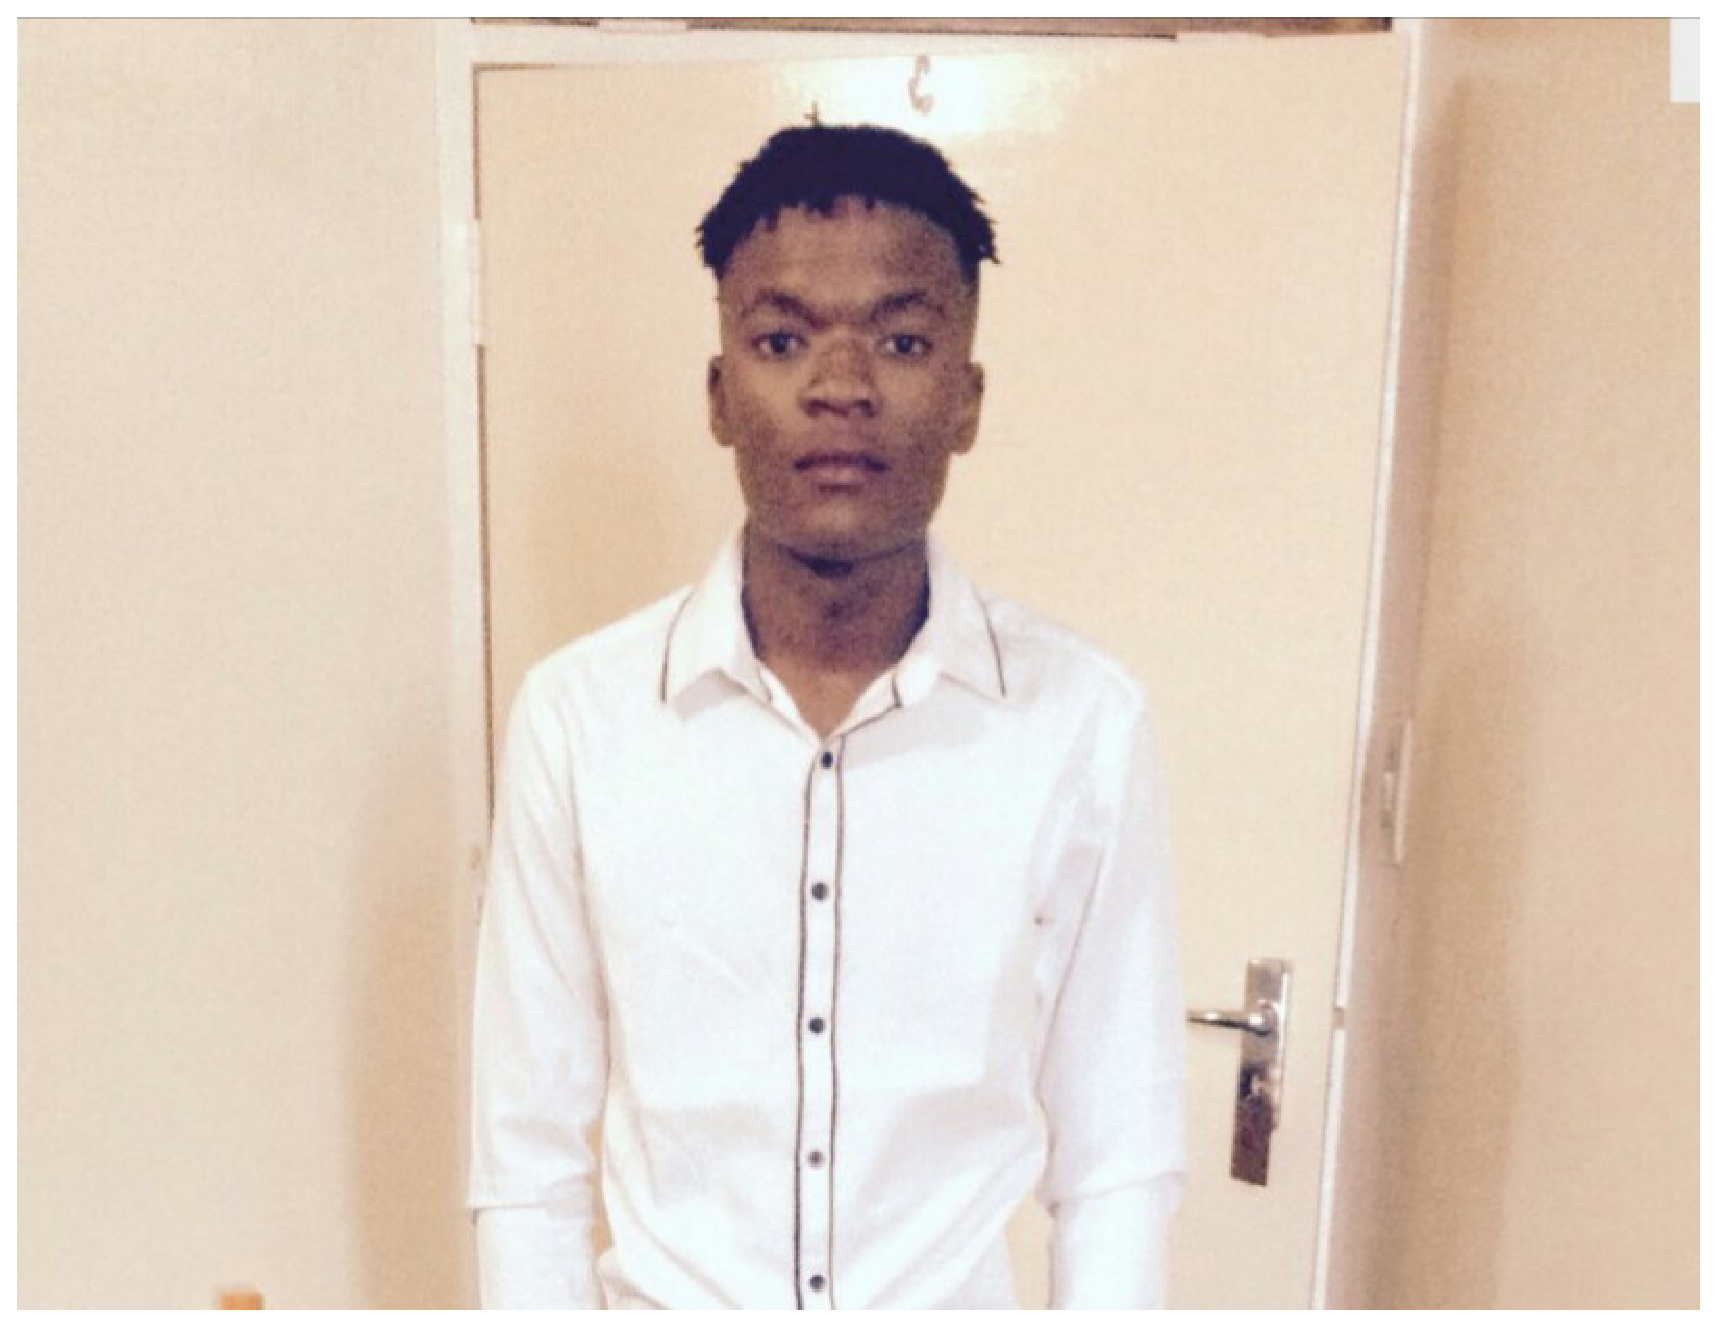
\includegraphics[width=5cm, height=5cm]{Oratile.eps} 
\end{figure}

 	\textit{To develop Caracal Automated Marking system, various interests and technical skills will be required, for example, being able to develop a system, work with different technologies and handle databases, also, programming skills and being able to code in multiple languages, and these are some of technical skills and interests I have listed above. Therefore, with team collaboration, and combination of common interests and skills, Caracal Automated Marking system will be interesting and fun to develop.}

\begin{center}
\begin{tabularx}{1.0\textwidth}{|p{3cm}|X|}
\hline
 {\LARGE Interests} & 
 \begin{compactitem}
     \item {\large System Design}
     \item {\large Databases}
     \item {\large Software Development}
	 \item {\large System Performance}
	 \item {\large Graphics (2D and 3D)}
 \end{compactitem} \\ 
 \hline
 {\LARGE Technical Skills} & 
 \begin{compactitem}
     \item {\large Programming / Scirpting / Coding, Object-Oriented Programmming}
     \item {\large Refactoring}
     \item {\large Flexible with mutliple languages (C#, C++, Java, Mark-up Languages and Query Languages)}
 \end{compactitem} \\ 
 \hline
 {\LARGE Past Experience} & 
 \begin{compactitem}
     \item {\large Developed a CCTV system that can monitor every action at the truck weigh scale and the system is also able take screenshots at any time and store them in a database.}
 \end{compactitem} \\ 
 \hline
 {\LARGE Non-Technical Skills} & 
 \begin{compactitem}
     \item {\large Communication}
     \item {\large Collaboration}
	 \item {\large Time Management}
	 \item {\large Creativity}
 \end{compactitem} \\
 \hline 
\end{tabularx}
\end{center}
\pagebreak
% Mankgwanyane Tlaka Profile ------------------------------------------------------------------
{\huge Mankgwanyane Tlaka}
\begin{figure}[h]
\centering
\includegraphics[width=5cm, height=5cm]{Mankgwanyane.eps} 
\end{figure}

 	\textit{I want to do this project because it is very innovative, creative, challenging and my type of work}

\begin{center}
\begin{tabularx}{1.0\textwidth}{|p{3cm}|X|}
\hline
 {\LARGE Interests} & 
 \begin{compactitem}
     \item {\large Data}
     \item {\large Optimazation}
     \item {\large Software Analysis and Modelling}
 \end{compactitem} \\ 
 \hline
 {\LARGE Technical Skills} & 
 \begin{compactitem}
     \item {\large Programming} 
     \item {\large Refactoring}
     \item {\large Flexible with mutliple languages}
 \end{compactitem} \\ 
 \hline
 {\LARGE Past Experience} & 
 \begin{compactitem}
     \item {\large I worked on the Comiar Project, which required for us to design and implement a course management system.}
     \item {\large I worked on an SRC electoral Project, which allowed students of the University of Pretoria to interact with the SRC candidates.}
	 \item {\large I worked on the NavUP system under the GIS module, which  required us to gather, maintain and persist information to navigate students around campus.}
 \end{compactitem} \\ 
 \hline
 {\LARGE Non-Technical Skills} & 
 \begin{compactitem}
     \item {\large Communication}
     \item {\large Leadership}
 \end{compactitem} \\
 \hline 
\end{tabularx}
\end{center}
\pagebreak
% Tlou Lebelo Profile ----------------------------------------------------------------
{\huge Tlou Lebelo}
\begin{figure}[h]
\centering
\includegraphics[width=5cm, height=5cm]{Tlou.eps} 
\end{figure}

 	\textit{I am interested in the field of Artificial Intelligence and the idea of having to develop a time efficient application that will be used in society for future developments.}

\begin{center}
\begin{tabularx}{1.0\textwidth}{|p{3cm}|X|}
\hline
 {\LARGE Interests} & 
 \begin{compactitem}
     \item {\large Advanced Learning in the field of Artificial Intelligence}
     \item {\large Mobile Application Software Development}
     \item {\large Using new software development tools and technologies}
 \end{compactitem} \\ 
 \hline
 {\LARGE Technical Skills} & 
 \begin{compactitem}
     \item {\large Coding (Object-Orientated Programming)} 
     \item {\large Coding(Java, C++, JavaScript, PHP}
     \item {\large Networking}
 \end{compactitem} \\ 
 \hline
 {\LARGE Past Experience} & 
 \begin{compactitem}
     \item {\large Community Based Project (JCP) - Installing computers for disadvantaged public high school in Pretoria CBD}
 \end{compactitem} \\ 
 \hline
 {\LARGE Non-Technical Skills} & 
 \begin{compactitem}
     \item {\large Team Work}
     \item {\large Good Mathematical Background}
     \item {\large Presentation Skills}
 \end{compactitem} \\
 \hline 
\end{tabularx}
\end{center}
\pagebreak
% Kenneth Mangwane Profile ------------------------------------------------------------------
{\huge Kenneth Mangwane}
\begin{figure}[h]
\centering
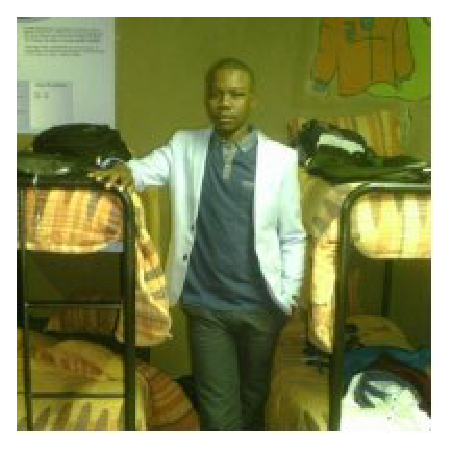
\includegraphics[width=5cm, height=5cm]{Kenneth.eps} 
\end{figure}

 	\textit{This project will assist a lot of teachers in marking scripts and I would love to be part of the team that revolutionizes marking.}

\begin{center}
\begin{tabularx}{1.0\textwidth}{|p{3cm}|X|}
\hline
 {\LARGE Interests} & 
 \begin{compactitem}
     \item {\large Machine Learning and Neural Networks}
     \item {\large Programming Languages}
     \item {\large Software Development}
     \item {\large Website Development}
 \end{compactitem} \\ 
 \hline
 {\LARGE Technical Skills} & 
 \begin{compactitem}
     \item {\large Programming in (C#, C, C++ and Java)} 
     \item {\large Scripting in (PHP, JavaScript and Bash)}
     \item {\large Mark-Up Language - HTML, XML, XSLT and WSDL}
     \item {\large Using Hosting Technologies and Hosting Websites}
 \end{compactitem} \\ 
 \hline
 {\LARGE Past Experience} & 
 \begin{compactitem}
     \item {\large Worked For Calibers IT Solutions as Technical and Web Designer}
     \item {\large Freelance Web Designer.}
 \end{compactitem} \\ 
 \hline
 {\LARGE Non-Technical Skills} & 
 \begin{compactitem}
     \item {\large Team work}
     \item {\large Listening}
     \item {\large Leadership}
 \end{compactitem} \\
 \hline 
\end{tabularx}
\end{center}
\pagebreak
%Team Section ------------------------------------------------------------------------
\section{Technologies}
Mathpix
  - PHP, SQL
  - openssl_encrypt / mcrypt
\Section{ Deployment Diagram}
\begin{figure}[h]
\centering
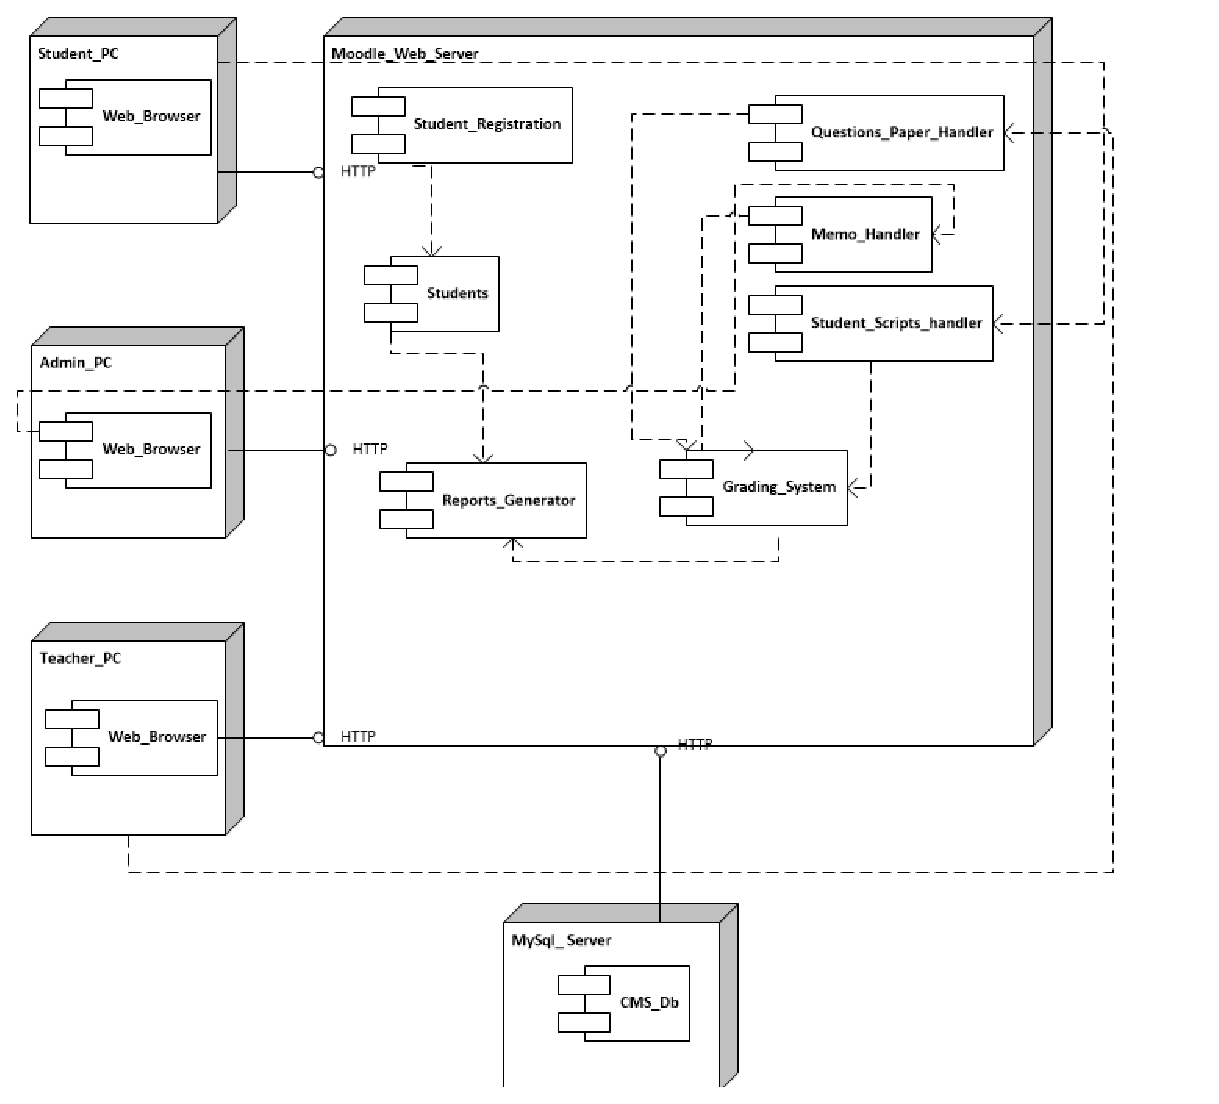
\includegraphics[width=12cm, height=12cm]{Caracal_Deployment_Diagram.eps} 
\end{figure}

\section{Development Methodology}

\section{Skills and Knowledge}

\end{document}
